\documentclass[a4paper,12pt]{article} 

%%% Работа с русским языком
\usepackage{cmap}					% поиск в PDF
\usepackage{mathtext} 				% русские буквы в фомулах
\usepackage[T2A]{fontenc}			% кодировка
\usepackage[utf8]{inputenc}			% кодировка исходного текста
\usepackage[english,russian]{babel}	% локализация и переносы

%%% Дополнительная работа с математикой
\usepackage{amsmath,amsfonts,amssymb,amsthm,mathtools, gensymb} % AMS
\usepackage{icomma} % "Умная" запятая: $0,2$    ф--- число, $0, 2$ --- перечисление

%%Таблица
\usepackage[table,xcdraw]{xcolor}
\usepackage{caption}
\usepackage{floatrow}
\floatsetup[table]{capposition=top}
\floatsetup[wrapfigure]{capposition=bottom}

%Отступы и поля 
\textwidth=18cm
\oddsidemargin=-1cm
\topmargin=-2cm
\textheight=25cm


%% Номера формул
\mathtoolsset{showonlyrefs=true} % Показывать номера только у тех формул, на которые есть \eqref{} в тексте.

%% Шрифты
\usepackage{euscript}	 % Шрифт Евклид
\usepackage{mathrsfs} % Красивый матшрифт

%% Свои команды
\DeclareMathOperator{\sgn}{\mathop{sgn}}

%% Перенос знаков в формулах (по Львовскому)
\newcommand*{\hm}[1]{#1\nobreak\discretionary{}
{\hbox{$\mathsurround=0pt #1$}}{}}

%% Стиль страницы
\usepackage{fancyhdr}

%% Для рисунков
\usepackage{graphicx}
\usepackage[export]{adjustbox}
\usepackage{float}
\usepackage{ragged2e}
\usepackage{wrapfig}

\pagestyle{fancy}
\begin{document}
\begin{titlepage}
\begin{center}
%\vspace*{1cm}
\large{\small ФЕДЕРАЛЬНОЕ ГОСУДАРСТВЕННОЕ АВТОНОМНОЕ ОБРАЗОВАТЕЛЬНОЕ\\ УЧРЕЖДЕНИЕ ВЫСШЕГО ОБРАЗОВАНИЯ \\ МОСКОВСКИЙ ФИЗИКО-ТЕХНИЧЕСКИЙ ИНСТИТУТ\\ (НАЦИОНАЛЬНЫЙ ИССЛЕДОВАТЕЛЬСКИЙ УНИВЕРСИТЕТ)\\ ФАКУЛЬТЕТ АЭРОКОСМИЧЕСКИХ ТЕХНОЛОГИЙ}
\vfill
\line(1,0){490}\\[1mm]
\huge{Лабораторная работа 3.6.1}\\
\huge\textbf{Спектральный анализ электрических сигналов}\\
\line(1,0){490}\\[1mm]
\vfill
\begin{flushright}
\normalsize{Рогозин Владимир}\\
\normalsize{\textbf{Группа Б03-106}}\\
\end{flushright}
\end{center}
\end{titlepage}
\fancyhead[L] {Работа 3.6.1}


\textbf{Цель работы}: 
изучить спектральный состав периодических электрических сигналов.

\textbf{Оборудование}:
цифровой анализатор спектра, генератор прямоугольных импульсов и сигналов специальной формы, осциллограф.

\textbf{Теоретические сведения}: 
В работе изучается спектральный состав периодических электрических сигналов различной формы: последовательности прямоугольных импульсов, последовательности цугов, амплитудно- и фазо-модулированных гармонических колебаний. Спектры этих сигналов наблюдаются с помощью анализатора спектра и сравниваются c рассчитанными теоретически.

Периодическая функция может быть представлена в виде бесконечного ряда гармонических функций -- ряда Фурье.
\[f(t) = \sum_{n = -\infty}^\infty c_n e^{i n \omega_0 t} \quad \text{или} \quad \sum_{n = 0}^\infty a_n \cos(n \omega_0 t + \varphi_n).\]
Где $\omega_0 = 2 \pi / T$, $T$ -- период функции $f(t)$. Коэффициенты \{$c_n$\} могут быть найдены по формуле 
\[c_n = \frac{1}{T} \int\limits_0^T f(t) e^{- i n \omega_0 t} dt.\]

Наборы коэффициентов разложения в комплексной \{$c_n$\} и действительной \{$a_n, \varphi_n$\} формах связаны соотношением 
\[a_n = 2 |c_n|, \quad \varphi_n = \text{arg }c_n.\]

\textbf{Экспериментальная установка}:
\begin{figure}[H]\label{fig: Ustanovka}
    \centering
    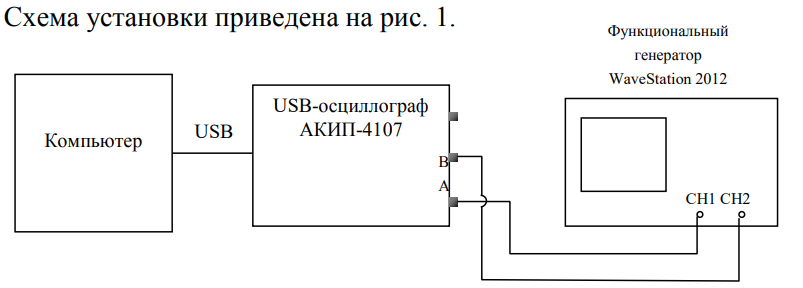
\includegraphics[width = 0.8\textwidth]{Установка.png}
     \caption{Экспериментальная установка}
\end{figure}

\textbf{Обработка данных}:  

\textbf{A. Исследование спектра периодической последовательности прямоугольных импульсов.}

Найдём спектр периодической последовательности прямоугольных импульсов длительности $\tau$ с периодом следования импульсов $T > \tau$ и значением $A$.
\[c_n = \frac{1}{T} \int\limits_{-\frac{\tau}{2}}^{\frac{\tau}{2}} A e^{-i n \omega_0 t} dt = A \cdot \frac{\sin(\pi n \tau / T)}{\pi n}.\]
График функции $c(\omega)$ будет выглядеть следующим образом
\begin{figure}[H]\label{fig: Pryamoug impulses spektr}
    \centering
    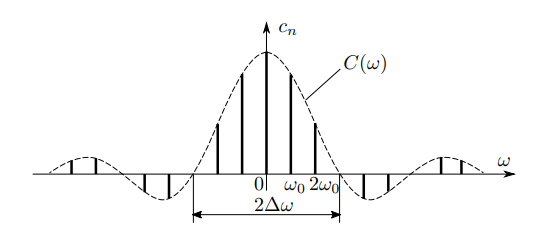
\includegraphics[width = 0.8\textwidth]{Прямоугольные импульсы.png}
    \caption{Спектр периодической последовательности прямоугольных импульсов}
\end{figure}
где $\Delta \omega = 2 \pi / \tau$. Основной вклад дают гармоники, частоты которых заполняют интервал $|\omega| < 2 \pi / \tau$. Этот диапазон частот можно назвать можно назвать характерной шириной спектра.

Сначала выставим частоту повторения импульсов $f_{повт} = 1$ кГц, длительность импульса $\tau = 100$ мкс. Проанализируем полученный спектр. 
\begin{figure}[H]\label{fig: 1kHz100mks}
    \centering
    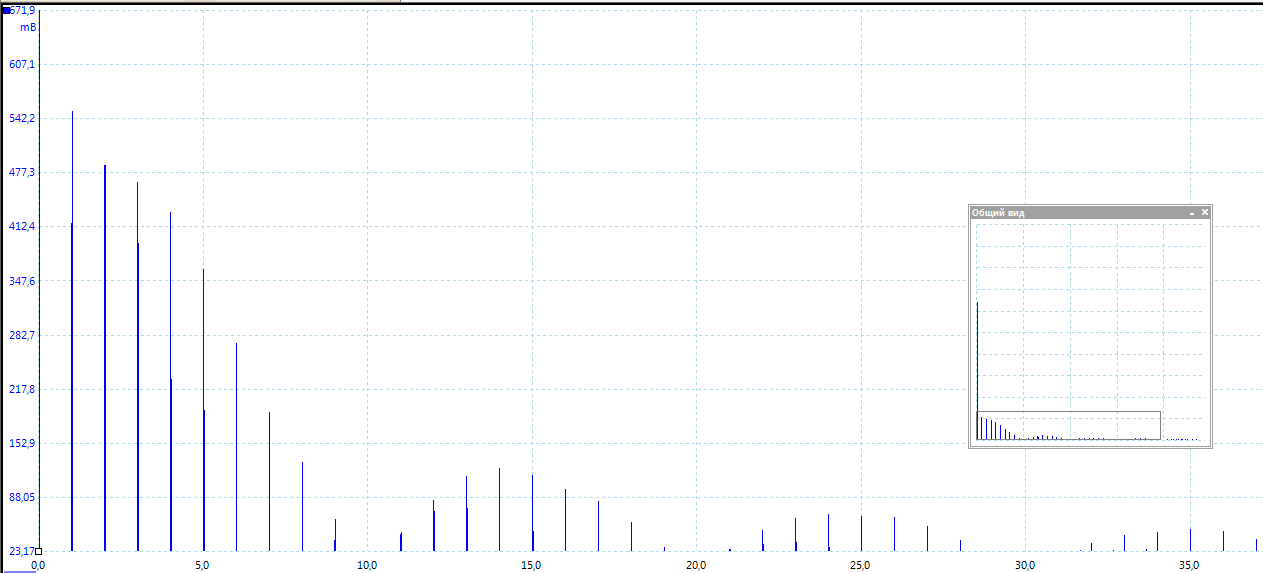
\includegraphics[width =\textwidth]{1kHz100mks.png}
    \caption{Спектр прямоугольных импульсов $T = 1$ мс; $\tau = 100$ мкс}
\end{figure}
Из картинки видно, что спектр совпадает с теорией, характерная ширина спектра $\Delta \nu$ равна $\tau^{-1} = 10$ кГц.

Далее уменьшим в два раза длину импульса и посторим на получившийся спектр. По сравнению с предыдущим случаем изменились амплитуды частот, а также увеличилась характерная ширина спектра $\Delta \nu = 20$ кГц.
\begin{figure}[H]\label{fig: 1kHz50mks}
    \centering
    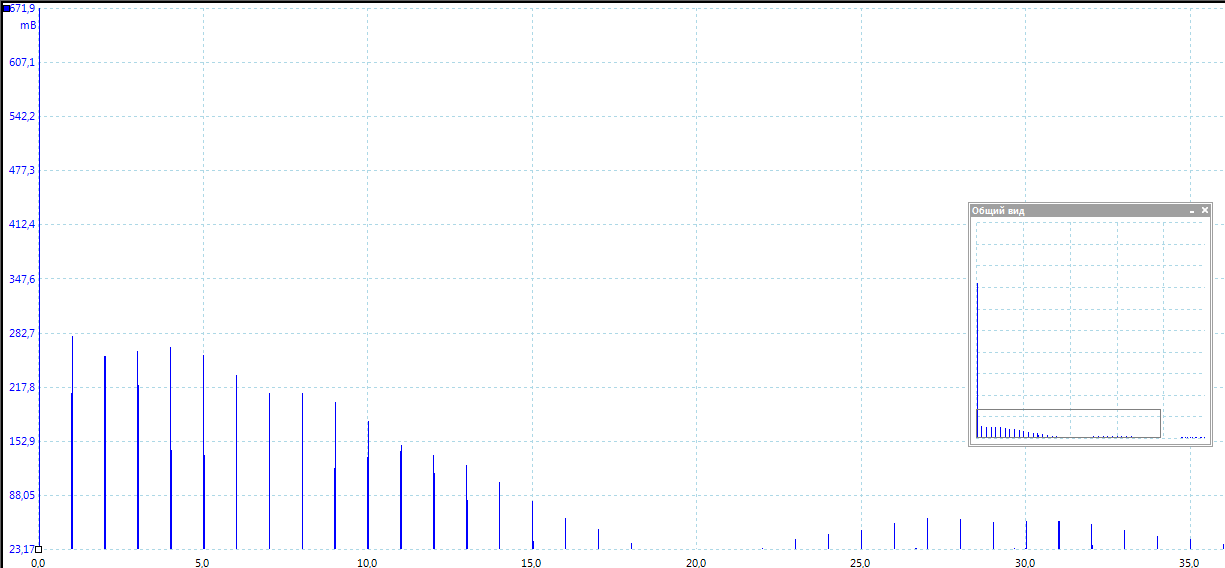
\includegraphics[width =\textwidth]{1kHz50mks.png}
    \caption{Спектр прямоугольных импульсов $T = 1$ мс; $\tau = 50$ мкс}
\end{figure}
Теперь изменим частоту сигнала до $f_{повт} = 2$ кГц при $\tau = 50$ мкс, посмотрим на спектр.
\begin{figure}[H]\label{fig: 2kHz50mks}
    \centering
    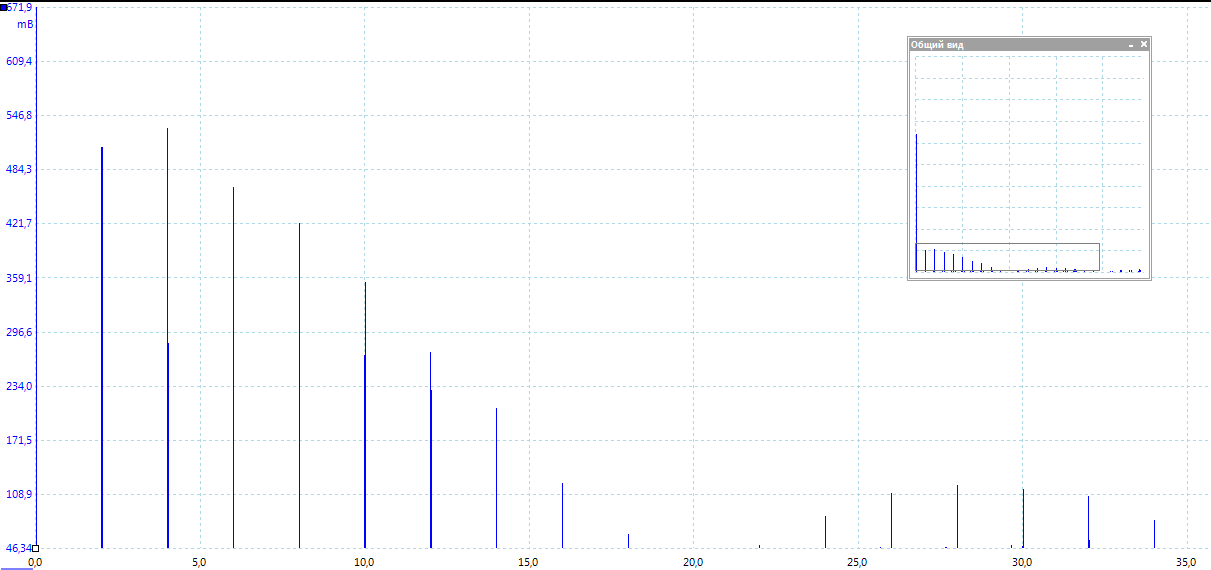
\includegraphics[width =\textwidth]{2kHz50mks.png}
    \caption{Спектр прямоугольных импульсов $T = 500$ мкс; $\tau = 50$ мкс}
\end{figure}
Как и следовало ожидать изменились амплитуды частот и частоты стали встерчаться реже, характерная ширина спектра осталась прежней.

Далее, при $f_{повт} = 1$ кГц снимем зависимость $\Delta \nu$ от $\tau$. По результатам построим график зависимости $\Delta \nu (1 / \tau)$. Данные представлены в таблице ниже.
\begin{table}[H]\label{tab: delta nu ot tau}
    \centering
    \begin{tabular}{|
        >{\columncolor[HTML]{FFFFFF}}c 
        >{\columncolor[HTML]{FFFFFF}}c 
        >{\columncolor[HTML]{FFFFFF}}c 
        >{\columncolor[HTML]{FFFFFF}}c 
        >{\columncolor[HTML]{FFFFFF}}c 
        >{\columncolor[HTML]{FFFFFF}}c 
        >{\columncolor[HTML]{FFFFFF}}c 
        >{\columncolor[HTML]{FFFFFF}}c 
        >{\columncolor[HTML]{FFFFFF}}c 
        >{\columncolor[HTML]{FFFFFF}}c 
        >{\columncolor[HTML]{FFFFFF}}c |}
        \hline
        \multicolumn{11}{|c|}{\cellcolor[HTML]{FFFFFF}{\color[HTML]{000000} $f_{повт} = 1$ кГц}} \\ \hline
        \multicolumn{1}{|c|}{\cellcolor[HTML]{FFFFFF}{\color[HTML]{000000} $\tau$, мкс}} &
          \multicolumn{1}{c|}{\cellcolor[HTML]{FFFFFF}{\color[HTML]{000000} 20}} &
          \multicolumn{1}{c|}{\cellcolor[HTML]{FFFFFF}{\color[HTML]{000000} 40}} &
          \multicolumn{1}{c|}{\cellcolor[HTML]{FFFFFF}{\color[HTML]{000000} 60}} &
          \multicolumn{1}{c|}{\cellcolor[HTML]{FFFFFF}{\color[HTML]{000000} 80}} &
          \multicolumn{1}{c|}{\cellcolor[HTML]{FFFFFF}{\color[HTML]{000000} 100}} &
          \multicolumn{1}{c|}{\cellcolor[HTML]{FFFFFF}{\color[HTML]{000000} 120}} &
          \multicolumn{1}{c|}{\cellcolor[HTML]{FFFFFF}{\color[HTML]{000000} 140}} &
          \multicolumn{1}{c|}{\cellcolor[HTML]{FFFFFF}{\color[HTML]{000000} 160}} &
          \multicolumn{1}{c|}{\cellcolor[HTML]{FFFFFF}{\color[HTML]{000000} 180}} &
          {\color[HTML]{000000} 200} \\ \hline
        \multicolumn{1}{|c|}{\cellcolor[HTML]{FFFFFF}{\color[HTML]{000000} $\Delta \nu$, кГц}} &
          \multicolumn{1}{c|}{\cellcolor[HTML]{FFFFFF}{\color[HTML]{000000} 50}} &
          \multicolumn{1}{c|}{\cellcolor[HTML]{FFFFFF}{\color[HTML]{000000} 25}} &
          \multicolumn{1}{c|}{\cellcolor[HTML]{FFFFFF}{\color[HTML]{000000} 17}} &
          \multicolumn{1}{c|}{\cellcolor[HTML]{FFFFFF}{\color[HTML]{000000} 12}} &
          \multicolumn{1}{c|}{\cellcolor[HTML]{FFFFFF}{\color[HTML]{000000} 10}} &
          \multicolumn{1}{c|}{\cellcolor[HTML]{FFFFFF}{\color[HTML]{000000} 8}} &
          \multicolumn{1}{c|}{\cellcolor[HTML]{FFFFFF}{\color[HTML]{000000} 7}} &
          \multicolumn{1}{c|}{\cellcolor[HTML]{FFFFFF}{\color[HTML]{000000} 6}} &
          \multicolumn{1}{c|}{\cellcolor[HTML]{FFFFFF}{\color[HTML]{000000} 5,5}} &
          {\color[HTML]{000000} 5} \\ \hline
        \end{tabular}
\caption{Данные измерений}
\end{table}


\textbf{Б. Исследование спектра периодической последовательности цугов гармонических колебаний.}

Последовательность цугов длиной $\tau$ и периодом $T > \tau$ можно представить в виде 
\[f(t) = f_0(t)\cos(\omega_0 t),\]
где $f_0(t)$ -- прямоугольный импульс длины $\tau$. Зная спектр прямоугольного импульса, можно изобразить спектр цуга. При домножении произвольной функции $g_0(t)$ на $e^{i \omega_0 t}$ спектр получившейся функции $g(t) = g_0(t)e^{i \omega_0 t}$ будет сдвинутым на величину $\omega_0$ вправо спектром функции $g_0(t)$. Поэтому спектр цуга может быть представлен следующим образом.
\begin{figure}[H]\label{fig: Zuch and impuls spektr}
    \centering
    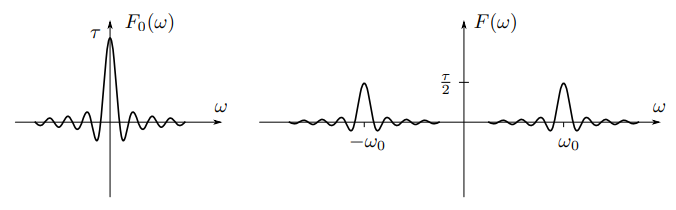
\includegraphics[width = \textwidth]{Импульс и цуг спектр.png}
    \caption{Спектры а) прямоугольного импульса и б) синусоидального цуга}
\end{figure}
Сгенерируем цуги и посмотрим на спектр такого сигнала при $T = 1$ мс, $\tau = 0,1$ мс, $\nu_0 = 50$ кГц, где $\nu_0$ -- частота синусоиды.
\begin{figure}[H]\label{fig: 50kHz_1ms_5N}
    \centering
    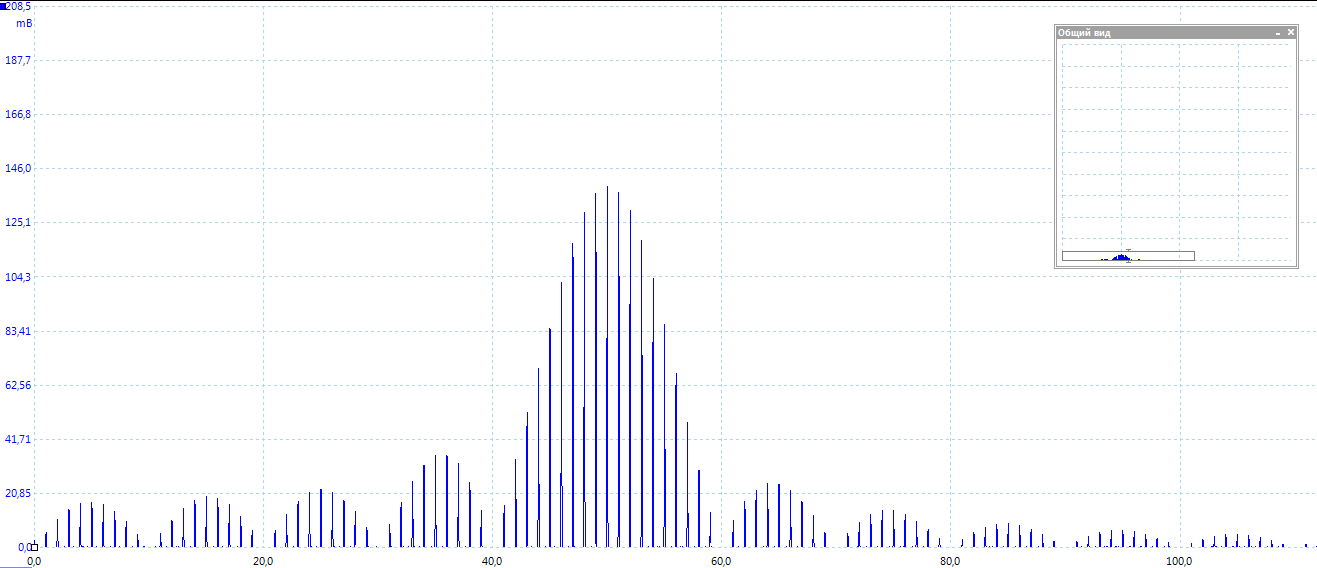
\includegraphics[width =\textwidth]{50kHz_1ms_5N.png}
    \caption{Спектр прямоугольных импульсов $T = 1$ мc; $\tau = 0,1$ мс; $\nu_0 = 50$ кГц}
\end{figure}
Получили в точности смещённый на 50 кГц спектр прямоугольного импульса.

Теперь увеличим период сигнала до 2 мс.
\begin{figure}[H]\label{fig: 50kHz_2ms_5N}
    \centering
    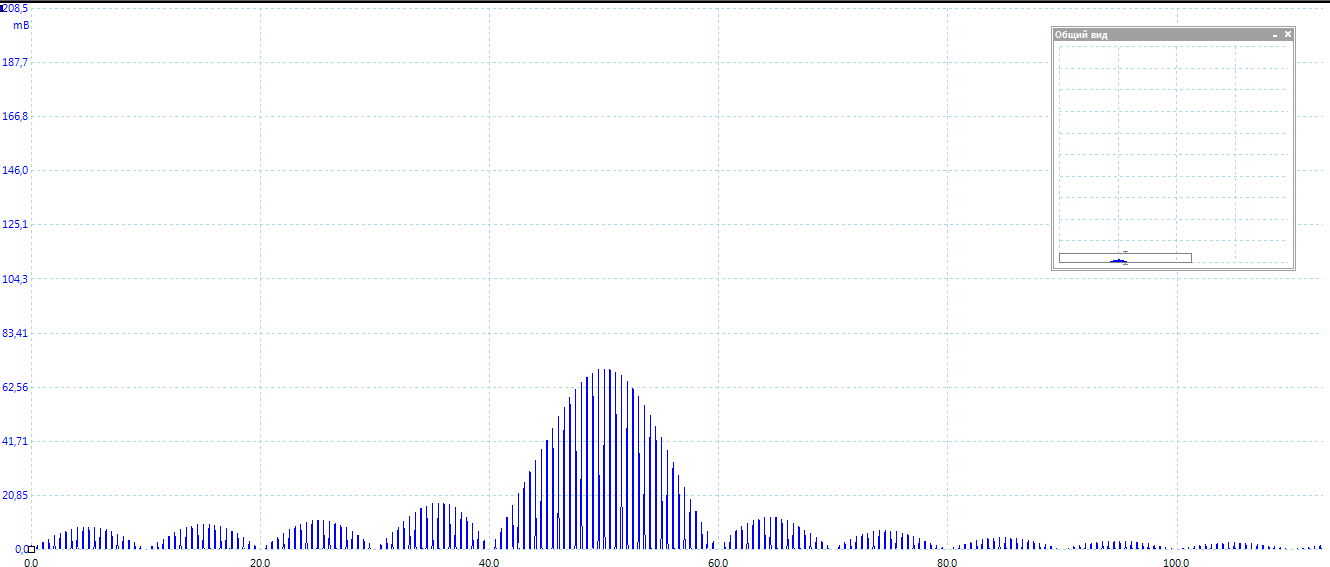
\includegraphics[width =\textwidth]{50kHz_2ms_5N.png}
    \caption{Спектр прямоугольных импульсов $T = 2$ мc; $\tau = 0,1$ мс; $\nu_0 = 50$ кГц}
\end{figure}
Частоты располагаются плотнее друг к другу чем в предыдущем случае.

Увеличим частоту синусоиды в два раза.
\begin{figure}[H]\label{fig: 100kHz_1ms_5N}
    \centering
    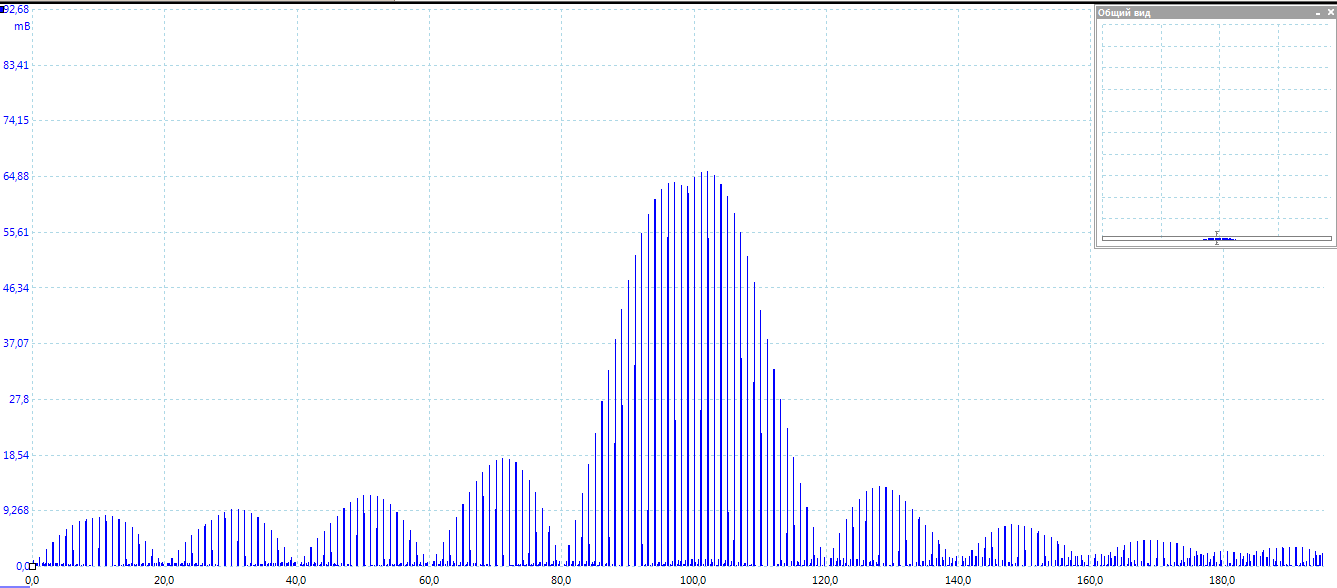
\includegraphics[width =\textwidth]{100kHz_1ms_5N.png}
        \caption{Спектр прямоугольных импульсов $T = 1$ мc; $\tau = 0,05$ мс; $\nu_0 = 100$ кГц}
\end{figure}
Центр спектра, как и предсказывает теория, сместился вправо на 50 кГц, характерная ширина спектра увеличилась вдвое. 

Увеличим длительность цуга до $\tau = 0,2$ мс. В результате видим сужение основного спектра.  
\begin{figure}[H]\label{fig: 50kHz_1ms_10N}
    \centering
    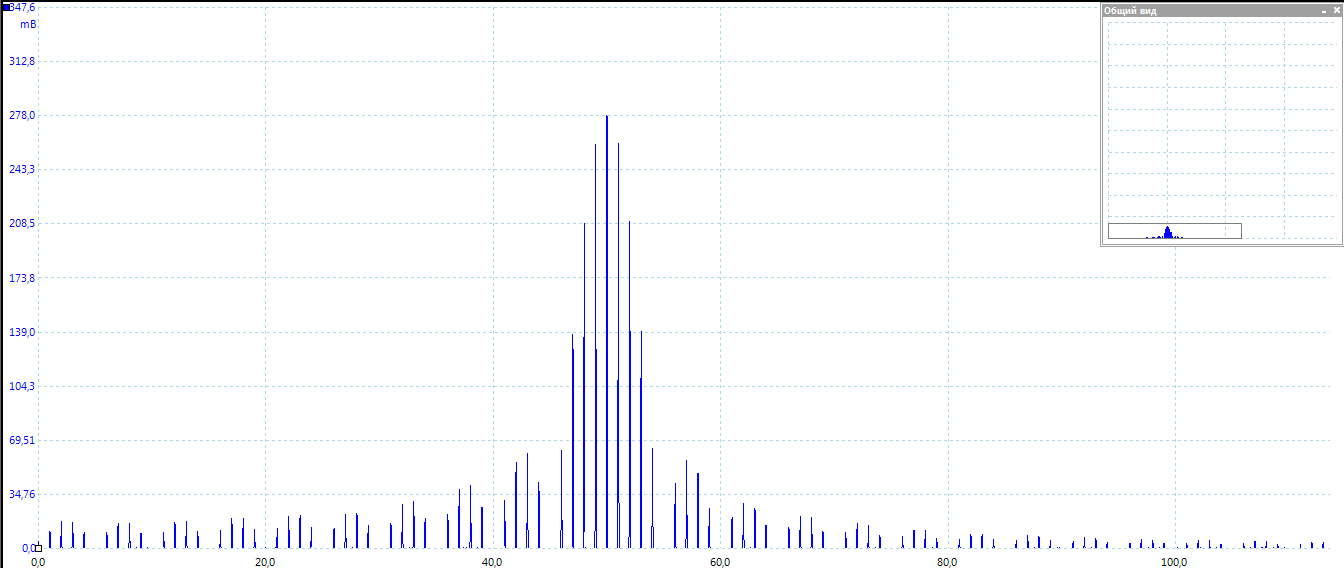
\includegraphics[width =\textwidth]{50kHz_1ms_10N.png}
        \caption{Спектр прямоугольных импульсов $T = 1$ мc; $\tau = 0,2$ мс; $\nu_0 = 50$ кГц}
\end{figure}

Увеличим частоту синусоиды вдвое, уменьшим длительность цуга вдвое.
\begin{figure}[H]\label{fig: 100kHz_1ms_10N}
    \centering
    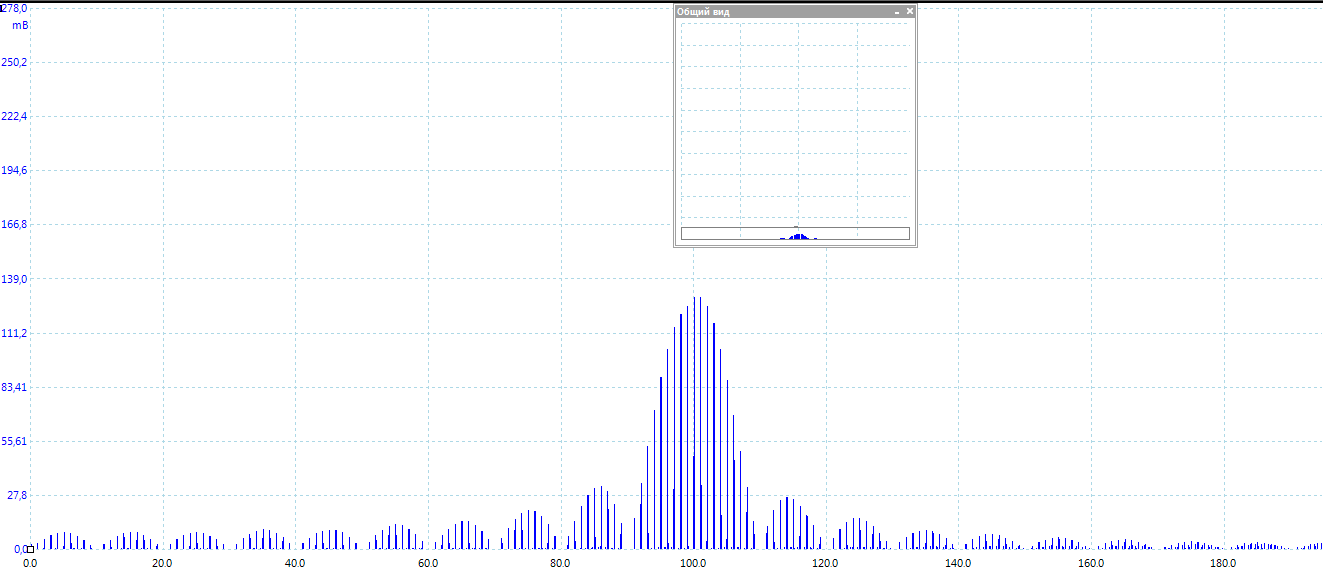
\includegraphics[width =\textwidth]{100kHz_1ms_10N.png}
        \caption{Спектр прямоугольных импульсов $T = 1$ мc; $\tau = 0,1$ мс; $\nu_0 = 100$ кГц}
\end{figure}

Теперь снимем зависимость $\delta \nu$ -- расстояния между соседними гармониками от частоты сигнала $f_{повт} = 1 / T$. По результатам измерений построим график зависимости $\delta \nu (1 / T)$. Данные представлены в таблице ниже.
\begin{table}[H]\label{tab: delta nu ot T}
    \centering
    \begin{tabular}{|
        >{\columncolor[HTML]{FFFFFF}}c 
        >{\columncolor[HTML]{FFFFFF}}c 
        >{\columncolor[HTML]{FFFFFF}}c 
        >{\columncolor[HTML]{FFFFFF}}c 
        >{\columncolor[HTML]{FFFFFF}}c 
        >{\columncolor[HTML]{FFFFFF}}c 
        >{\columncolor[HTML]{FFFFFF}}c 
        >{\columncolor[HTML]{FFFFFF}}c 
        >{\columncolor[HTML]{FFFFFF}}c 
        >{\columncolor[HTML]{FFFFFF}}c 
        >{\columncolor[HTML]{FFFFFF}}c 
        >{\columncolor[HTML]{FFFFFF}}c 
        >{\columncolor[HTML]{FFFFFF}}c 
        >{\columncolor[HTML]{FFFFFF}}c |}
        \hline
        \multicolumn{14}{|c|}{\cellcolor[HTML]{FFFFFF}{\color[HTML]{000000} $\nu = 50$ кГц, $N = 5$}} \\ \hline
        \multicolumn{1}{|c|}{\cellcolor[HTML]{FFFFFF}{\color[HTML]{000000} $1 / f_{повт} = T$, мс}} &
          \multicolumn{1}{c|}{\cellcolor[HTML]{FFFFFF}{\color[HTML]{000000} 0,2}} &
          \multicolumn{1}{c|}{\cellcolor[HTML]{FFFFFF}{\color[HTML]{000000} 0,4}} &
          \multicolumn{1}{c|}{\cellcolor[HTML]{FFFFFF}{\color[HTML]{000000} 0,6}} &
          \multicolumn{1}{c|}{\cellcolor[HTML]{FFFFFF}{\color[HTML]{000000} 0,8}} &
          \multicolumn{1}{c|}{\cellcolor[HTML]{FFFFFF}{\color[HTML]{000000} 1,0}} &
          \multicolumn{1}{c|}{\cellcolor[HTML]{FFFFFF}{\color[HTML]{000000} 1,5}} &
          \multicolumn{1}{c|}{\cellcolor[HTML]{FFFFFF}{\color[HTML]{000000} 2,0}} &
          \multicolumn{1}{c|}{\cellcolor[HTML]{FFFFFF}{\color[HTML]{000000} 2,5}} &
          \multicolumn{1}{c|}{\cellcolor[HTML]{FFFFFF}{\color[HTML]{000000} 3,0}} &
          \multicolumn{1}{c|}{\cellcolor[HTML]{FFFFFF}{\color[HTML]{000000} 3,5}} &
          \multicolumn{1}{c|}{\cellcolor[HTML]{FFFFFF}{\color[HTML]{000000} 4,0}} &
          \multicolumn{1}{c|}{\cellcolor[HTML]{FFFFFF}{\color[HTML]{000000} 4,5}} &
          {\color[HTML]{000000} 5,0} \\ \hline
        \multicolumn{1}{|c|}{\cellcolor[HTML]{FFFFFF}{\color[HTML]{000000} $\delta \nu$, кГц}} &
          \multicolumn{1}{c|}{\cellcolor[HTML]{FFFFFF}{\color[HTML]{000000} 9,95}} &
          \multicolumn{1}{c|}{\cellcolor[HTML]{FFFFFF}{\color[HTML]{000000} 2,55}} &
          \multicolumn{1}{c|}{\cellcolor[HTML]{FFFFFF}{\color[HTML]{000000} 1,681}} &
          \multicolumn{1}{c|}{\cellcolor[HTML]{FFFFFF}{\color[HTML]{000000} 1,25}} &
          \multicolumn{1}{c|}{\cellcolor[HTML]{FFFFFF}{\color[HTML]{000000} 1,0}} &
          \multicolumn{1}{c|}{\cellcolor[HTML]{FFFFFF}{\color[HTML]{000000} 0,67}} &
          \multicolumn{1}{c|}{\cellcolor[HTML]{FFFFFF}{\color[HTML]{000000} 0,5}} &
          \multicolumn{1}{c|}{\cellcolor[HTML]{FFFFFF}{\color[HTML]{000000} 0,4}} &
          \multicolumn{1}{c|}{\cellcolor[HTML]{FFFFFF}{\color[HTML]{000000} 0,34}} &
          \multicolumn{1}{c|}{\cellcolor[HTML]{FFFFFF}{\color[HTML]{000000} 0,28}} &
          \multicolumn{1}{c|}{\cellcolor[HTML]{FFFFFF}{\color[HTML]{000000} 0,24}} &
          \multicolumn{1}{c|}{\cellcolor[HTML]{FFFFFF}{\color[HTML]{000000} 0,22}} &
          {\color[HTML]{000000} 0,2} \\ \hline
    \end{tabular}
    \caption{Данные измерений}
\end{table}


\textbf{В. Исследование спектра гармонических сигналов, модулированных по амплитуде.}

Для передачи сигналов -- музыки, речи, телевизионного изображения -- необходимо нарушение синусоидальности. Отклонение от синусоидальности и выражает содержание передаваемой информации. Колебательный процесс, отличный от гармонического, называется \textit{модулированным колебанием}.
\begin{figure}[H]\label{fig: Modulation examples}
    \centering
    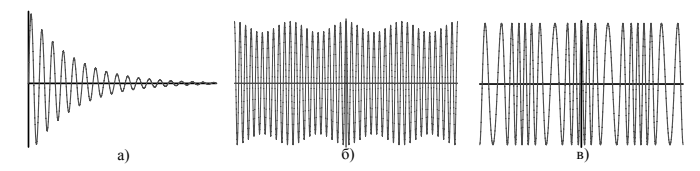
\includegraphics[width = \textwidth]{Примеры модуляций.png}
    \caption{Примеры модулированных колебаний: а, б) -- по амплитуде, в) -- по фазе}
\end{figure}

В общем случае модулированные колебания записываются в виде
\[f(t) = a(t) \cos(\omega_0 t + \varphi (t)).\]
Если $\tau \gg T$, где $\tau$ -- характерное время изменения амплитуды $a(t)$ и фазы $\varphi (t)$, то такие колебания называются \textit{квазигармоническими}. В этом случае медленно меняющиеся величины $a(t)$ и $\varphi (t)$ принято называть \textit{амплитудой} и \textit{начальной фазой} модулированного колебания соответственно.

Для описания модулированных колебаний используется следующая терминология: говорят, что функция $a(t)$ описывает закон амплитудной модуляции, а функция $\varphi (t)$ -- закон фазовой модуляции. Именно в этих функциях и может быть заложена передаваемая информация.

Если $\varphi (t) = \varphi_0 = const$, то такое колебание называют \textit{модулированным по амплитуде}. Простейший случай амплитудно-модулированного колебания -- в котором амплитуда модуляции является гармонической функцией.
\[f(t) = a(t)\cos \omega_0 t, \quad \text{ где} \quad a(t) = a_0(1 + m\cos\Omega t).\]
Константа $0 < m \leq 1$ называется \textit{глубиной модуляции}. Глубину модуляции можно выразить через максимальную $a_{max}$ и минимальную $a_{min}$ амплитуды сигнала:
\begin{equation}\label{eq: m via amax amin}
   m = \frac{a_{max} - a_{min}}{a_{max} + a_{min}}. 
\end{equation}

Преобразовав выражение для $f(t)$, получим соотношение
\[f(t) = a_0 \cos \omega_0 t + \frac{m a_0}{2} \cos(\omega_0 + \Omega) t + \frac{m a_0}{2} \cos(\omega_0 - \Omega) t.\]
Итак, амплитудно-модулированное по гармоническому закону колебание представляется в виде суммы трёх гармонических колебаний:
\[f_0(t) = a_0 \cos \omega_0 t, \text{  } f_1(t) = \frac{m a_0}{2} \cos(\omega_0 + \Omega) t, \text{  } f_2(t) = \frac{m a_0}{2} \cos(\omega_0 - \Omega) t.\]
Колебание $f_0(t)$ называется \textit{несущим колебанием}, а $f_1(t)$ и $f_2(t)$ -- \textit{боковыми гармониками}. 

Проанализируем спектры амлитудно-модулированных сигналов при разных несущих и боковых частотах, а также различных глубинах модуляции.
\begin{figure}[H]\label{fig: nu_AM_25kHz_nu_0}
    \centering
    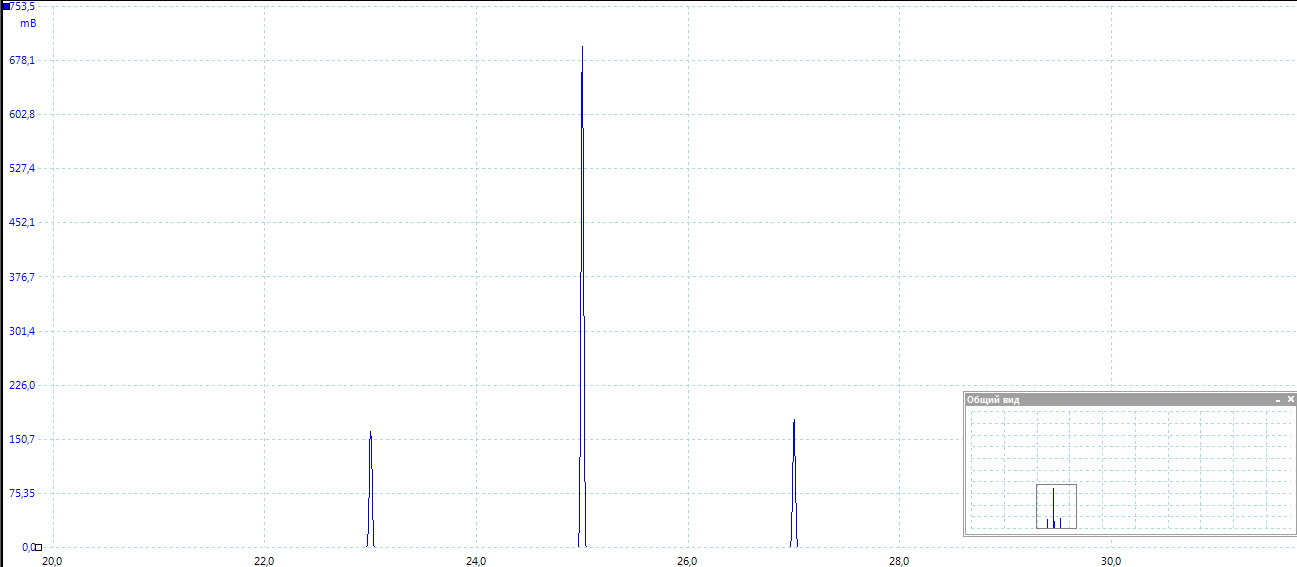
\includegraphics[width = \textwidth]{nu_AM_25kHz_nu_0.png}
    \caption{$f_{нес} = 25$ кГц, $f_{мод} = 2$ кГц, $m = 0,5$}
\end{figure}
Как и должно быть, видим несущую гармонику на частоте $\nu = 25$ кГц и две боковых на частотах ($\nu = 25 \pm 2$) кГц.
\begin{figure}[H]\label{fig: nu_AM_50kHz_nu_0}
    \centering
    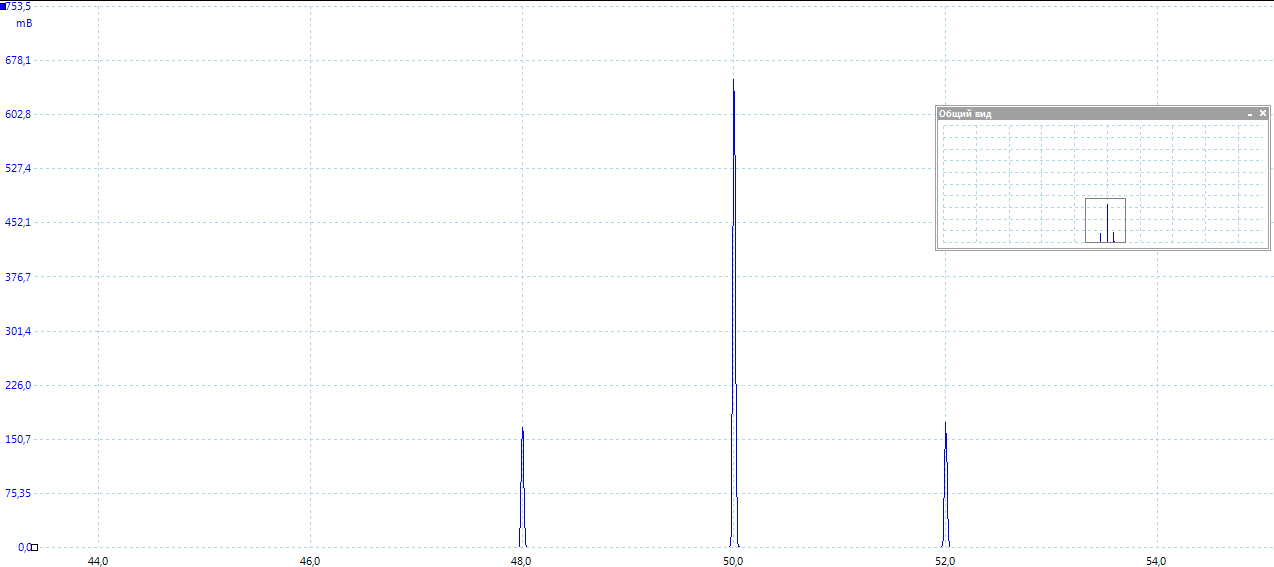
\includegraphics[width = \textwidth]{nu_AM_50kHz_nu_0.png}
    \caption{$f_{нес} = 50$ кГц, $f_{мод} = 2$ кГц, $m = 0,5$}
\end{figure}
Теперь несущая гармоника находится на частоте 50 кГц, боковые ($50 \pm 2$) кГц.

\begin{figure}[H]\label{fig: nu_AM_50kHz_nu_4kHz}
    \centering
    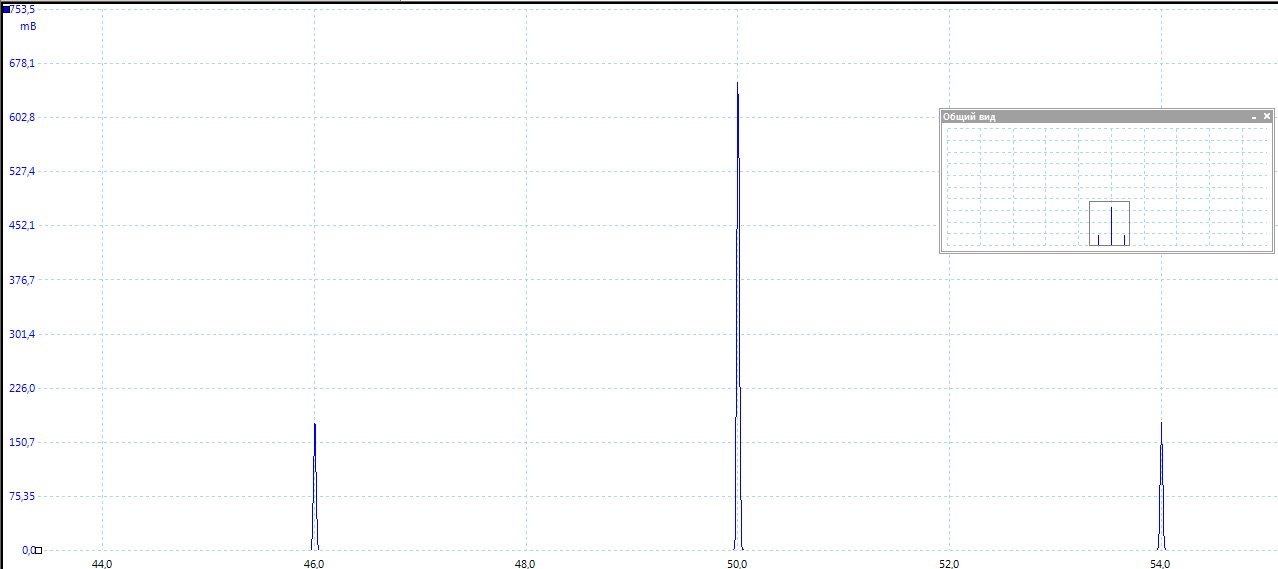
\includegraphics[width = \textwidth]{nu_AM_50kHz_nu_mod.png}
    \caption{$f_{нес} = 50$ кГц, $f_{мод} = 4$ кГц, $m = 0,5$}
\end{figure}
В этом случае несущая гармоника на такой же частоте, что и в предыдущем случае, боковые ($50 \pm 4$) кГц.

Также, при $m_{теор} = 0,5$, запишем значения $a_{max} = 1529$ ед., $a_{min} = 515,5$ ед., и проверим справедливость формулы  \eqref{eq: m via amax amin}.
\[m_{эксп} = 0,496 \approx m_{теор} = 0,5.\]
Получаем совпадение с хорошей точностью.

Далее снимем зависимость отношения амплитуд боковой и несущей гармоник от глубины модуляции.
\begin{table}[H]\label{tab: a_b and a_o ot m}
    \centering
    \begin{tabular}{|
        >{\columncolor[HTML]{FFFFFF}}c |
        >{\columncolor[HTML]{FFFFFF}}c |
        >{\columncolor[HTML]{FFFFFF}}c |
        >{\columncolor[HTML]{FFFFFF}}c |
        >{\columncolor[HTML]{FFFFFF}}c |
        >{\columncolor[HTML]{FFFFFF}}c |
        >{\columncolor[HTML]{FFFFFF}}c |
        >{\columncolor[HTML]{FFFFFF}}c |
        >{\columncolor[HTML]{FFFFFF}}c |
        >{\columncolor[HTML]{FFFFFF}}c |
        >{\columncolor[HTML]{FFFFFF}}c |}
        \hline
        {\color[HTML]{000000} $m$} &
          {\color[HTML]{000000} 0,1} &
          {\color[HTML]{000000} 0,2} &
          {\color[HTML]{000000} 0,3} &
          {\color[HTML]{000000} 0,4} &
          {\color[HTML]{000000} 0,5} &
          {\color[HTML]{000000} 0,6} &
          {\color[HTML]{000000} 0,7} &
          {\color[HTML]{000000} 0,8} &
          {\color[HTML]{000000} 0,9} &
          {\color[HTML]{000000} 1,0} \\ \hline
        {\color[HTML]{000000} $a_{бок}$, ед.} &
          {\color[HTML]{000000} 32,76} &
          {\color[HTML]{000000} 65,52} &
          {\color[HTML]{000000} 99,71} &
          {\color[HTML]{000000} 133,9} &
          {\color[HTML]{000000} 168,1} &
          {\color[HTML]{000000} 202,3} &
          {\color[HTML]{000000} 236,5} &
          {\color[HTML]{000000} 267,8} &
          {\color[HTML]{000000} 303,4} &
          {\color[HTML]{000000} 334,1} \\ \hline
        {\color[HTML]{000000} $a_{осн}$, ед.} &
          {\color[HTML]{000000} 658,1} &
          {\color[HTML]{000000} 662,3} &
          {\color[HTML]{000000} 669,0} &
          {\color[HTML]{000000} 659,5} &
          {\color[HTML]{000000} 660,9} &
          {\color[HTML]{000000} 658,1} &
          {\color[HTML]{000000} 659,5} &
          {\color[HTML]{000000} 659,5} &
          {\color[HTML]{000000} 659,5} &
          {\color[HTML]{000000} 655,2} \\ \hline
    \end{tabular}
    \caption{Данные измерений $a_{осн}$ и $a_{бок}$ при различных $m$}
\end{table}
По данным с таблицы построим график зависимости $a_{бок} / a_{осн}$ от $m$, проанализируем совпадение с теорией.

\textbf{Г. Исследование спектра гармонических сигналов, модулированных по фазе.}

Рассмотрим теперь простейший пример фазовой модуляции:
\[f(t) = a_0 \cos(\omega_0 t + \varphi (t)), \quad \text{ где } \varphi (t) = m \cos \Omega t.\]
Константа $m$ -- \textit{глубина модуляции фазы} -- определяет диапазон
изменения начальной фазы.

В общем случае закон модуляции приводит к довольно сложному спектру, поэтому рассмотрим случай $m \ll 1$. Тогда, после нескольких преобразований, получим
\[f(t) = a_0 \cos \omega_0 t + \frac{m a_0}{2} \cos\bigg((\omega_0 + \Omega) t + \frac{\pi}{2}\bigg) + \frac{m a_0}{2} \cos\bigg((\omega_0 - \Omega) t + \frac{\pi}{2}\bigg).\]
\begin{figure}[H]\label{fig: Amplitude and phase modul spektr}
    \centering
    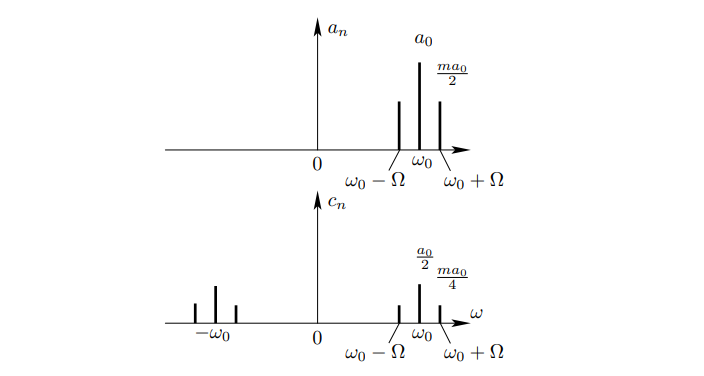
\includegraphics[width = 0.9\textwidth]{Амплитудно и фазо-модулированный спектр.png}
    \caption{Спектр колебаний, модулированных гармонически по фазе или амплитуде. Действительное (вверху) и комплексное (внизу) представления}
\end{figure}

Амплитудно-частотная характеристика обоих сигналов одинаковая, но сами сигналы сильно различаются. Всё дело в фазово-частотной характеристике, которая будет различна для этих сигналов. Из формул видно, что боковые гармоники отличаются фазовым сдвигом на $\frac{\pi}{2}$. Отсюда понятно, что чтобы восстановить сигнал мало знать амплитуды спектральных компонент, нужно  ещё иметь информацию об их фазах.

Посмотрим на спектры сигналов, модулированных по фазе, с малой глубиной модуляции $m \ll 1$. Будем изменять величины $\omega_0$, $\Omega$ и $\varphi$ и смотреть как меняется спектр.
\begin{figure}[H]\label{fig: nu_PM_50kHz_phi_20}
    \centering
    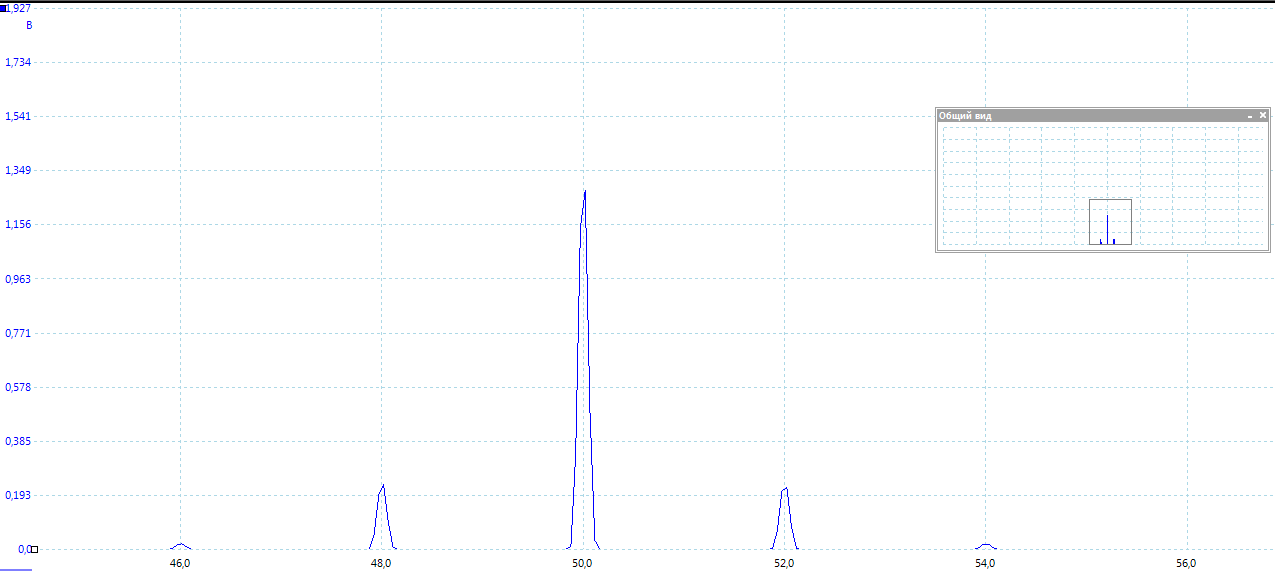
\includegraphics[width = \textwidth]{nu_PM_50kHz_phi_20.png}
    \caption{$f_{нес} = 50$ кГц, $f_{мод} = 2$ кГц, $\varphi = 20\degree$}
\end{figure}
Видим, что спектр очень схож со спектром амлитудно-модулированного сигнала, но появляются дополнительные гармоники, которых в теории при $m \rightarrow 0$ не должно быть.

\begin{figure}[H]\label{fig: nu_PM_50kHz_phi_10}
    \centering
    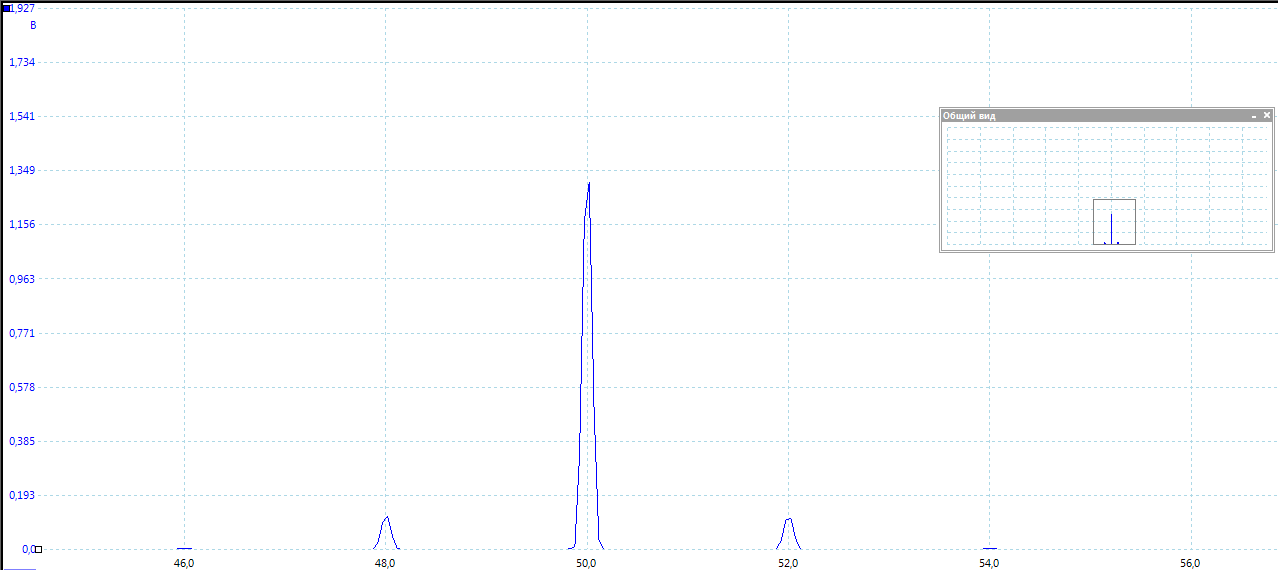
\includegraphics[width = \textwidth]{nu_PM_50kHz_phi_10.png}
    \caption{$f_{нес} = 50$ кГц, $f_{мод} = 2$ кГц, $\varphi = 10\degree$}
\end{figure}
\begin{figure}[H]\label{fig: nu_PM_25kHz_phi_10}
    \centering
    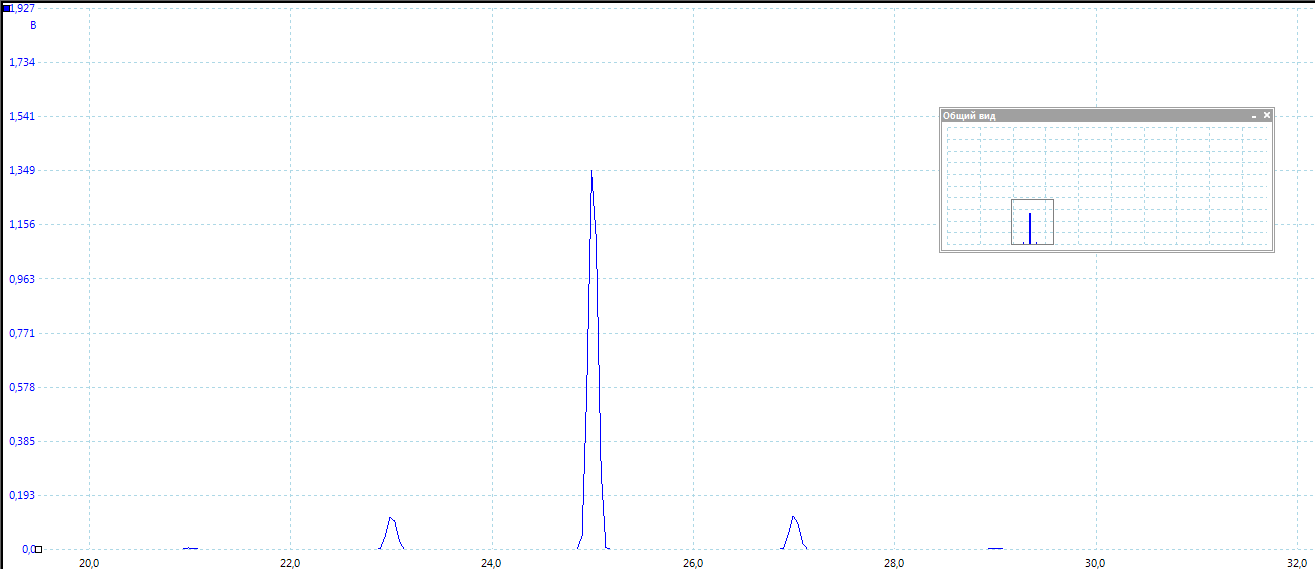
\includegraphics[width = \textwidth]{nu_PM_25kHz.png}
    \caption{$f_{нес} = 25$ кГц, $f_{мод} = 2$ кГц, $\varphi = 10\degree$}
\end{figure}


\begin{figure}[H]\label{fig: nu_PM_50kHz_nu_4kHz}
    \centering
    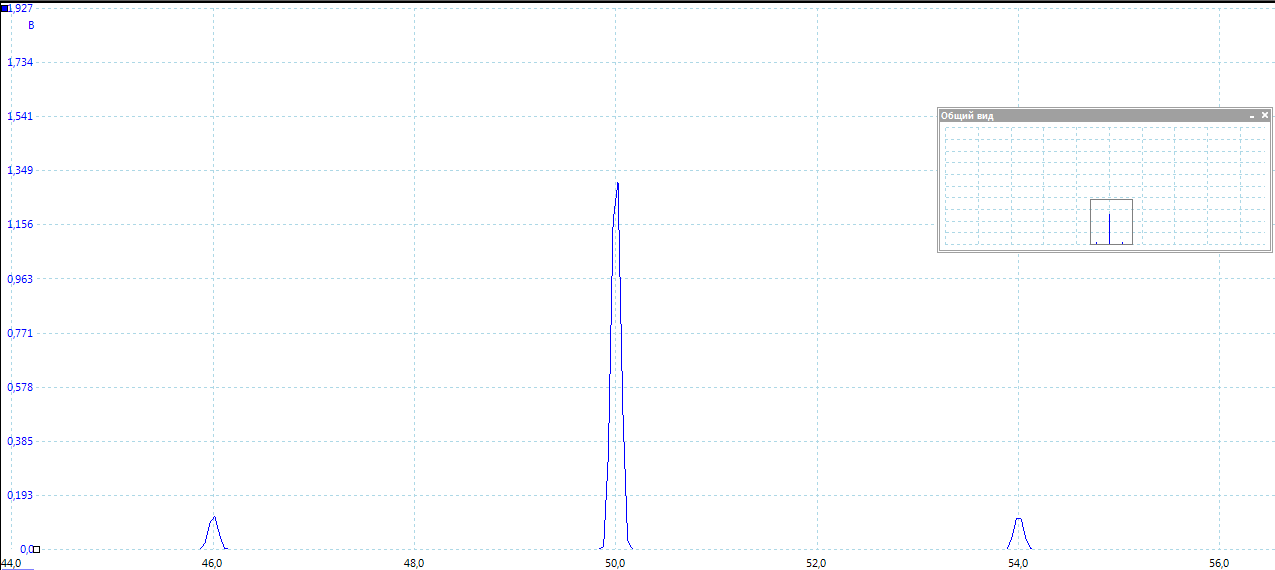
\includegraphics[width = \textwidth]{nu_PM_50kHz_nu_4kHz.png}
    \caption{$f_{нес} = 50$ кГц, $f_{мод} = 4$ кГц, $\varphi = 10\degree$}
\end{figure}
\begin{figure}[H]\label{fig: nu_PM_25kHz_phi_20_nu_2kHz}
    \centering
    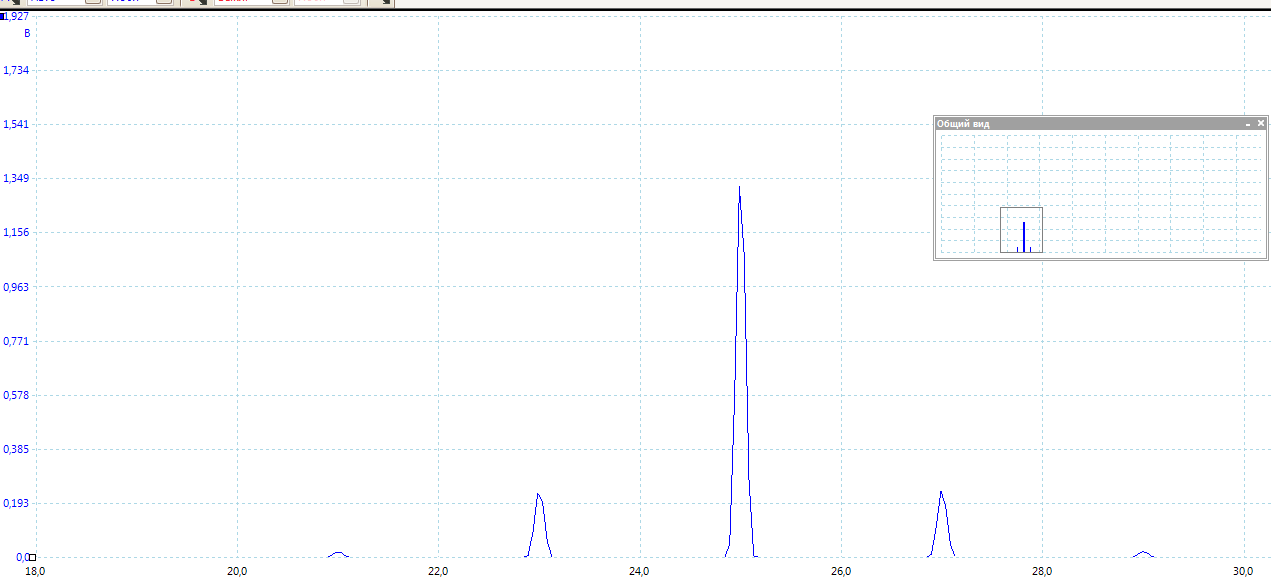
\includegraphics[width = \textwidth]{nu_PM_25kHz_phi_20_nu_2kHz.png}
    \caption{$f_{нес} = 25$ кГц, $f_{мод} = 2$ кГц, $\varphi = 20\degree$}
\end{figure}

\textbf{Вывод}:

%%%%%%%%%%%%%%%%%%%%%%%%% Графики
\newpage
\begin{figure}[H]\label{fig: Delta_nu(1 / tau)}
    \centering
    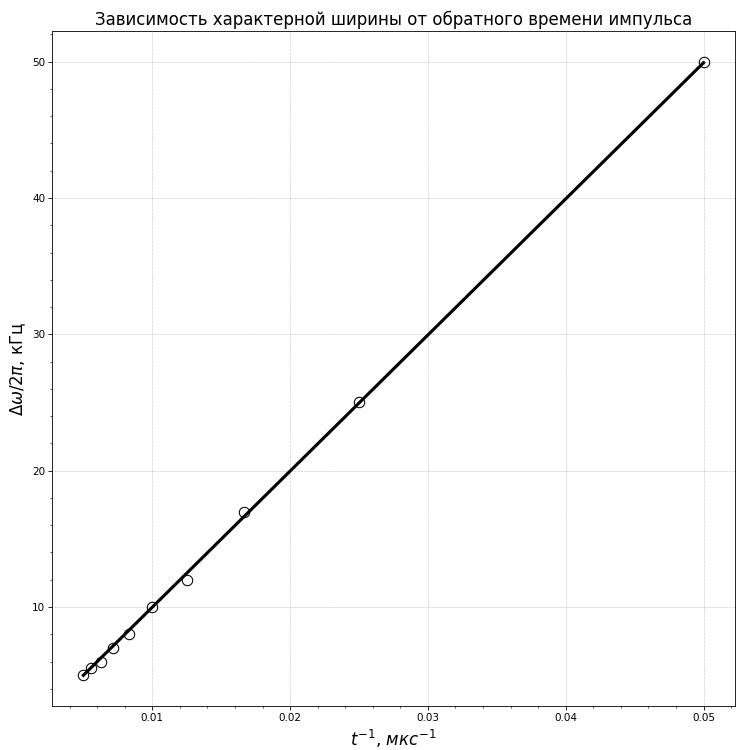
\includegraphics[width = \textwidth]{Delta_nu(tau pow-1).png}
\end{figure}
\[k = \frac{\Delta \omega \cdot \Delta t}{2 \pi} = 0,998 \pm 0,004; \quad \varepsilon_k = 0,38\%\]
Следовательно получаем $\Delta \omega \cdot \Delta t \approx 2 \pi$, что и подтверждает соотношение неопределённостей.

\newpage
\begin{figure}[H]\label{fig: delta_nu(1 / T)}
    \centering
    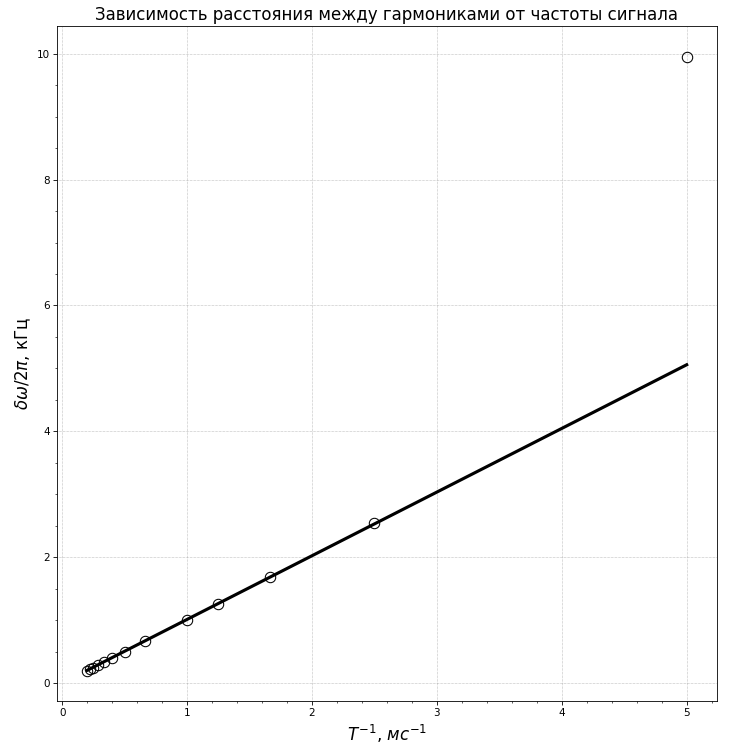
\includegraphics[width = \textwidth]{delta_nu(T pow-1).png}
\end{figure}
При аппроксимации были учтены все точки кроме самой первой ($T = 0,2$ мс).
\[k = 1,012 \pm 0,003; \quad \varepsilon_k = 0,27\%\]
При этом теоретическая зависимость имеет вид $\Delta \nu \cdot T = 1$, что хорошо подтверждается экспериментом.

\newpage
\begin{figure}[H]\label{fig: a_b div a_o (m)}
    \centering
    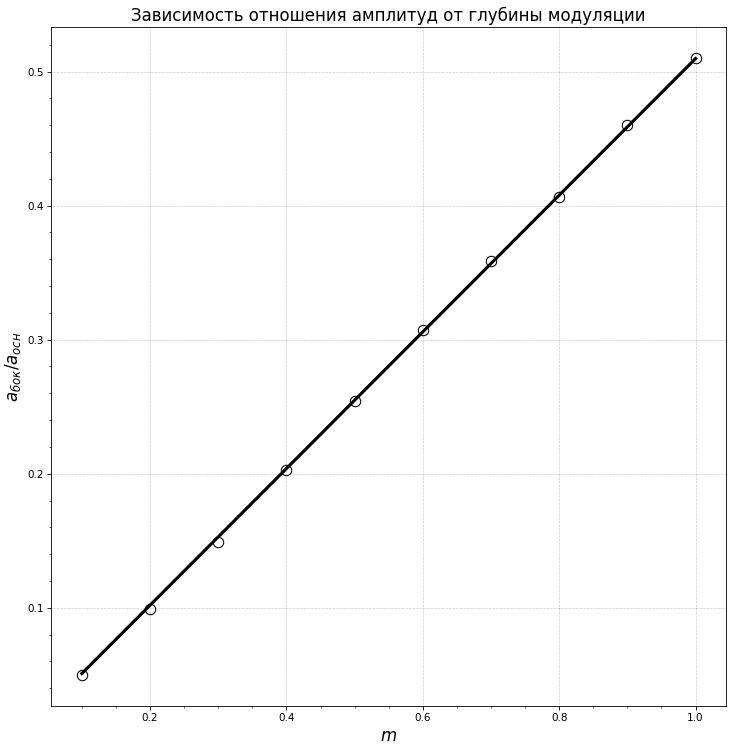
\includegraphics[width = \textwidth]{a_b div a_o (m).png}
\end{figure}
\[k = 0,510 \pm 0,001; \quad \varepsilon_k = 0,19\%\]
Теоретическая оценка даёт зависимость
\[\frac{a_{бок}}{a_{осн}} = \frac{1}{2} m,\]
что с хорошей точностью совпадает с полученной экспериментально.


%%%%%%%%%%%%%%%%%%%%%%%%%
\end{document}
